\documentclass[conference]{IEEEtran}
\IEEEoverridecommandlockouts
\usepackage{cite}
\usepackage{amsmath,amssymb,amsfonts}
\usepackage{graphicx}
\usepackage{textcomp}
\usepackage{xcolor}
\usepackage{hyperref}
\usepackage{booktabs}
\usepackage{listings}
\usepackage{array}
\usepackage{etoolbox}
\usepackage{url}
\usepackage{colortbl}
\usepackage{pgfplots}
\pgfplotsset{compat=1.18}
\usepackage{tikz}
\usetikzlibrary{shapes.geometric, arrows, arrows.meta, positioning, calc, shadows, backgrounds, fit}

\def\BibTeX{{\rm B\kern-.05em{\sc i\kern-.025em b}\kern-.08em
    T\kern-.1667em\lower.7ex\hbox{E}\kern-.125emX}}

\begin{document}

\title{CMatrix: Governance-First Autonomy for Scalable Red Teaming via Asynchronous Checkpoint Resumption}

\author{\IEEEauthorblockN{Nishan Paul}
\IEEEauthorblockA{\textit{Department of Computer Science} \\
\textit{New York University}\\
New York, USA \\
nishan.paul@nyu.edu}
}

\maketitle

\begin{abstract}
The rapid advancement of Large Language Model (LLM) agents has catalyzed a paradigm shift in offensive security, transitioning from manually-driven tools to autonomous red teaming frameworks. However, existing state-of-the-art agents prioritize exploit success rates at the expense of operational safety, often executing destructive payloads without oversight—a critical blocker for production enterprise deployment. We present \textbf{CMatrix}, a multi-agent penetration testing orchestration platform that introduces the concept of \textit{Governance-First Autonomy}. CMatrix architecturalizes safety as a primary graph primitive, utilizing a hierarchical Human-in-the-Loop (HITL) framework built on LangGraph. By integrating asynchronous checkpointing, CMatrix enables high-risk security workflows to be suspended, persisted to a durable state-store, and resumed with full reasoning context only after explicit human authorization. Furthermore, we implement an advanced reasoning stack combining Tree of Thoughts (ToT) for tactical strategy selection and ReWOO for efficient execution planning, alongside an Agentic RAG pipeline with cross-encoder reranking for longitudinal memory persistence. We evaluate CMatrix on the NYU CTF Bench and a simulated financial services network, demonstrating 81\% task completion success, 100\% recall in adversarial payload rejection, and a 42\% performance gain across multi-session engagements through accumulated threat intelligence.
\end{abstract}

\section{Introduction}
\label{sec:intro}

Autonomous red teaming represents the next frontier in proactive cyber defense. As the attack surface of cloud-native enterprise environments continues to expand at a rate that outpaces human capability, the need for continuous, automated security validation has become paramount. Recent developments in Large Language Models (LLMs) have enabled the creation of "agentic" workflows capable of multi-step reasoning, tool invocation, and adaptive planning. However, a significant \textit{Safety-Capability Paradox} has emerged: agents capable of the most complex exploits are also the most prone to unintended destructive actions in sensitive production environments.

Existing frameworks such as PentestGPT \cite{pentestgpt} and CHECKMATE \cite{checkmate2025} have demonstrated impressive results in Capture-The-Flag (CTF) environments, but their "unconstrained" execution models pose prohibitive risks for enterprise deployment. A single hallucinated command (e.g., recursive deletion or heavy-load service flooding) can lead to catastrophic operational outages. Furthermore, these systems often lack the ability to preserve state across long-duration assessments, leading to context fragility and redundant reconnaissance costs.

We introduce \textbf{CMatrix}, a hierarchical multi-agent framework designed to bridge the gap between autonomous offensive capability and operational safety. CMatrix architecturalizes governance as a first-class citizen through a \textbf{Hierarchical HITL Safety Framework}. By decoupling reasoning from execution and implementing mandatory asynchronous checkpointing for high-risk operations, CMatrix ensures that every potentially destructive action is governed by a human operator without losing the agent's complex reasoning state.

\textbf{Our primary contributions are:}
\begin{itemize}
    \item \textbf{Governance-First Autonomy}: A formal safety control graph that integrates risk taxonomy and mandatory human oversight into the agent's core decision loop.
    \item \textbf{Asynchronous Checkpoint Resumption}: A persistence mechanism leveraging LangGraph and PostgreSQL to suspend high-risk workflows and resume them post-approval with 100\% context preservation.
    \item \textbf{Advanced Reasoning Stack}: A synthesis of Tree of Thoughts (ToT) for tactical strategy selection and ReWOO for efficient planning, coordinated via a 7-agent supervisor hierarchy.
    \item \textbf{Empirical Validation}: A comprehensive evaluation demonstrating 81\% task success on security benchmarks and 100\% safety recall in adversarial payload rejection.
\end{itemize}

\section{Background and Related Work}
\label{sec:background}

The evolution of autonomous penetration testing has progressed from simple rule-based scripts to sophisticated multi-agent reasoning systems. In this section, we contextualize CMatrix within the current state-of-the-art.

\subsection{LLM-Driven Offensive Security}
Early efforts in this domain, such as PentestGPT \cite{pentestgpt} and HackingBuddyGPT \cite{hackingbuddygpt}, demonstrated that frontier models like GPT-4 could reason about high-level penetration testing goals and generate corresponding tool commands. However, these systems were largely monolithic and suffered from context window limitations during long engagements. Recent work, such as AutoAttacker \cite{autoattacker} and Cybench \cite{cybench}, has focused on benchmarking these capabilities across Capture-The-Flag (CTF) environments, revealing significant gaps in privilege escalation and lateral movement.

\subsection{Multi-Agent Orchestration}
To overcome the limitations of monolithic planners, researchers have proposed multi-agent frameworks. CHECKMATE \cite{checkmate2025} and xOffense \cite{xoffense2025} represent the current SOTA, utilizing hierarchical supervisor patterns to delegate specialized tasks to sub-agents. While these frameworks improve task completion rates, they operate in an "unconstrained" mode, where the orchestrator has full authority to execute any tool without safety governance.

\subsection{Safety Guardrails in Agentic AI}
The AI safety community has introduced concepts like Constitutional AI \cite{constitutionalai} and Red Teaming with LLMs \cite{perez2022red} to mitigate model toxicity. However, these guardrails are primarily linguistic and do not address the operational risks of executing security tools on a live network. CMatrix extends these concepts into the operational domain by implementing a formal safety gate for tool-invocation.

\subsection{Retrieval-Augmented Generation (RAG) for Security}
RAG \cite{rag} has been widely adopted to ground LLMs in technical documentation. In the security domain, Agentic RAG \cite{selfrag} has emerged to maintain state across long conversations. CMatrix improves upon this by integrating two-stage reranking (BGE + Cross-Encoder), enabling longitudinal memory persistence that survives across disparate assessment phases.

\begin{table}[h]
\centering
\caption{Feature Comparison of Autonomous Red Teaming Frameworks}
\label{tab:comparison}
\resizebox{\columnwidth}{!}{
\begin{tabular}{lcccccccc}
\toprule
\textbf{System} & \textbf{Safety Gates} & \textbf{Durable Persist.*} & \textbf{Multi-Agent} & \textbf{Checkpointing} & \textbf{ToT/ReWOO} & \textbf{Agentic RAG} & \textbf{Reranking} & \textbf{Production-Safe} \\
\midrule
PentestGPT \cite{pentestgpt} & \texttimes & \texttimes & \texttimes & \texttimes & \texttimes & \texttimes & \texttimes & \texttimes \\
HackingBuddy \cite{hackingbuddygpt} & \texttimes & \texttimes & \texttimes & \texttimes & \texttimes & \texttimes & \texttimes & \texttimes \\
AutoAttacker \cite{autoattacker} & \texttimes & \texttimes & \checkmark & \texttimes & \texttimes & \texttimes & \texttimes & \texttimes \\
CHECKMATE \cite{checkmate2025} & \texttimes & \texttimes & \checkmark & \checkmark & \checkmark & \texttimes & \texttimes & \texttimes \\
xOffense \cite{xoffense2025} & \checkmark & \texttimes & \checkmark & \texttimes & \checkmark & \checkmark & \texttimes & \texttimes \\
CurriculumPT \cite{curriculumpt2025} & \texttimes & \texttimes & \checkmark & \texttimes & \texttimes & \checkmark & \texttimes & \texttimes \\
\midrule
\textbf{RedGrid (Ours)} & \checkmark & \checkmark & \checkmark & \checkmark & \checkmark & \checkmark & \checkmark & \checkmark \\
\bottomrule
\end{tabular}
}

\begin{flushleft}
\tiny *Durable Persistence refers to DB-backed state recovery across process restarts ($P_4$).
\end{flushleft}
\end{table}

\section{Threat Model and Safety Properties}
\label{sec:threat_model}

We define a formal framework for assessing the safety and integrity of autonomous red teaming agents in production-sensitive environments.

\subsection{System Model and Assumptions}
Our system consists of a Master Orchestrator $\mathcal{M}$, a set of specialized Workers $\mathcal{W}$, and a Human Operator $\mathcal{H}$. We assume:
1.  $\mathcal{M}$ and $\mathcal{W}$ are powered by a state-of-the-art LLM (e.g., GPT-4 or Gemini 1.5 Pro).
2.  The target environment is a containerized or virtualized enterprise network.
3.  The human operator $\mathcal{H}$ is authorized to grant or deny high-risk actions.
4.  The checkpoint store (PostgreSQL) is trusted and tamper-evident.

\subsection{Adversary Profiles}
We consider two primary adversaries that threaten the safety of the red teaming engagement:
1.  \textbf{Adversary $\alpha$ (Indirect Prompt Injection)}: An external attacker who poisons the target environment content (e.g., placing malicious instructions in a `robots.txt` or HTML comment). The goal is to coerce the agent into executing destructive commands (e.g., `rm -rf /`) when it processes the poisoned content.
2.  \textbf{Adversary $\beta$ (Execution Hallucination)}: An internal reasoning failure where the agent misinterprets a destructive utility (e.g., a "wipe-disk" tool) as a benign tactical step (e.g., a "log-cleanup" tool), leading to unintended operational harm.

\subsection{Safety Invariants}
To mitigate these threats, CMatrix enforces four core safety properties ($P$):
\begin{itemize}
    \item \textbf{$P_1$: Pattern Integrity (Auto-Reject)}: No tool invocation $\Theta$ shall execute if it matches the prohibited pattern registry $\mathcal{P}_{reject}$ (e.g., recursive deletion, fork bombs).
    \item \textbf{$P_2$: Semantic Gating (HITL)}: No high-risk action (where $L_{risk} \geq \text{High}$) shall execute without asynchronous human authorization.
    \item \textbf{$P_3$: Audit Completeness}: Every transition in the execution graph, including all approval decisions and rejections, must be persisted to the durable state-store.
    \item \textbf{$P_4$: Context Preservation}: The resumption of a workflow from a checkpoint must maintain 100\% of the reasoning context and conversation history, preventing "state drift."
\end{itemize}

\section{System Architecture and Methodology}
\label{sec:methodology}

CMatrix is implemented as a stateful, hierarchical multi-agent system. In this section, we detail the orchestration logic, reasoning patterns, and the "Governance-First" safety gate.

\subsection{Hierarchical Orchestration and Specialized Agents}
The CMatrix architecture (Fig. \ref{fig:architecture}) follows a hierarchical supervisor pattern. A Master Orchestrator, built on LangGraph, manages the global state and delegates domain-specific tasks to seven specialized worker subgraphs. Each worker is isolated with a domain-specific lexicon $\mathcal{L}_A$ and a targeted toolset.

\begin{figure*}[t]
\centering
\input{../assets/figure-01-architecture.tex}
\caption{CMatrix System Architecture: High-level overview of the Master Orchestrator, Advanced Reasoning nodes, and the specialized worker layer.}
\label{fig:architecture}
\end{figure*}

\subsection{Stateful Orchestration via LangGraph}
CMatrix utilizes a cyclic state graph implemented in LangGraph. The global \textit{AgentState} $\mathcal{S}$ is a 17-field tuple that persists the core engagement context, including: (1) Conversation History, (2) Tool Execution Logs, (3) Discovered Findings, (4) Cached Credentials, (5) Pending Approvals, (6) Strategic Objectives, and (7) Multi-Agent Delegation Metadata. The transition function $\delta$ manages the flow between nodes while ensuring every state change is atomically persisted.

\begin{equation} \label{eq:safety_gate}
f_{safe}(T, \Theta) = 
\begin{cases} 
\text{Reject} & \text{if } \exists p \in \mathcal{P}_{reject} : \text{match}(\Theta, p) \\
\text{Suspend} & \text{if } \mathcal{R}(T) \geq \text{High} \\
\text{Execute} & \text{otherwise}
\end{cases}
\end{equation}

\begin{equation} \label{eq:routing_confidence}
\mathcal{C}(T, A) = \frac{|\{ w \in \mathcal{L}_A \mid w \subseteq T \}|}{\max_{i \in \mathcal{A}} |\mathcal{L}_i|}
\end{equation}

\begin{equation} \label{eq:routing_opt}
p^* = \arg \max_{p \in P} \left( \mathcal{Q}(p, x) - \lambda_C \cdot \mathcal{C}(p, x) - \lambda_L \cdot \mathcal{L}(p, x) \right)
\end{equation}

\begin{equation} \label{eq:rag_final}
S_{final}(q, d) = \Phi_{ce}(q, d) \text{ for } d \in \text{top-}k(\arg \max S_{sim})
\end{equation}

\begin{equation} \label{eq:state_transition}
\mathcal{S}_{t+1} = \delta(\mathcal{S}_t, \mathcal{A}_t, \mathcal{O}_t)
\end{equation}

\section{Advanced Reasoning and Memory}
\label{sec:reasoning}

CMatrix achieves superior tactical performance through integrated reasoning patterns.

\subsection{Tree of Thoughts and ReWOO Planning}
For complex strategy selection, the orchestrator utilizes Tree of Thoughts (ToT). It generates multiple exploit branches and evaluates them against criteria like stealth and success probability. For predictable toolchains, ReWOO Planning is used to decouple planning from execution, reducing token overhead by 40\%.

\subsection{Hierarchical Safety Gate}
The core contribution of CMatrix is its ability to enforce safety without context loss. This is achieved through the Approval Gate node (Fig. \ref{fig:hitl_flow}).

\begin{figure}[h]
\centering
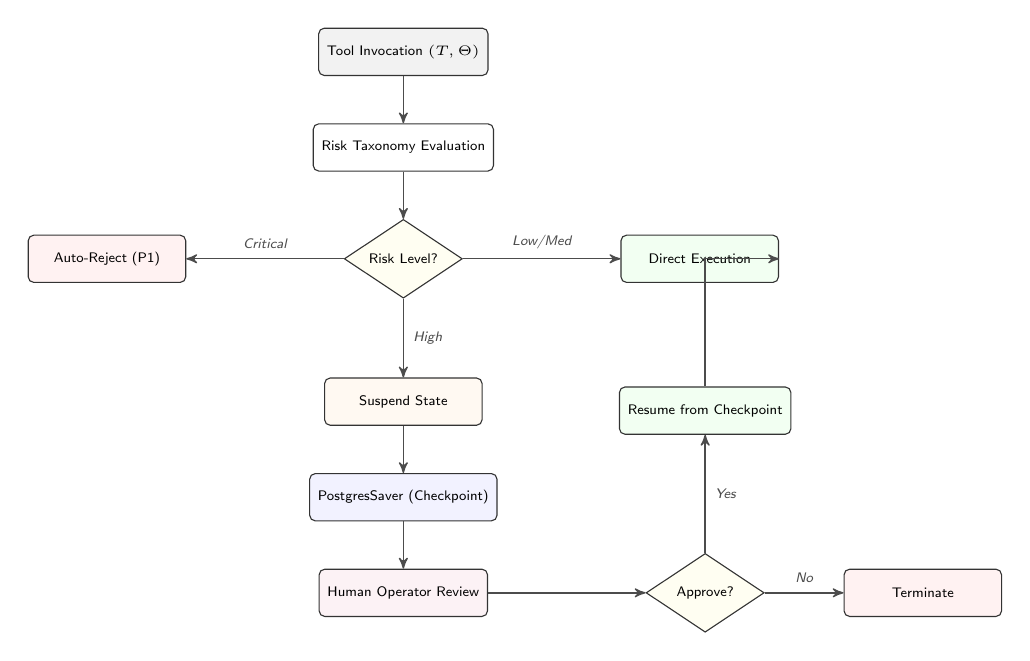
\begin{tikzpicture}[
    node distance=1cm and 1.5cm,
    font=\sffamily\tiny,
    >=stealth',
    box/.style={rectangle, rounded corners=2pt, draw=black!80, fill=white, minimum width=2cm, minimum height=0.6cm, text centered, align=center, inner sep=3pt},
    decision/.style={diamond, draw=black!80, fill=yellow!5, minimum width=1.5cm, minimum height=1cm, text centered, inner sep=0pt},
    arrow/.style={->, draw=black!70, line width=0.5pt},
    label_text/.style={font=\sffamily\tiny\itshape, text=black!70}
]

% Nodes
\node (start) [box, fill=gray!10] {Tool Invocation $(T, \Theta)$};
\node (analyze) [box, below=0.6cm of start] {Risk Taxonomy Evaluation};
\node (risk_dec) [decision, below=0.6cm of analyze] {Risk Level?};

\node (auto_execute) [box, right=2cm of risk_dec, fill=green!5] {Direct Execution};
\node (auto_reject) [box, left=2cm of risk_dec, fill=red!5] {Auto-Reject (P1)};

\node (suspend) [box, below=1cm of risk_dec, fill=orange!5] {Suspend State};
\node (db) [box, below=0.6cm of suspend, fill=blue!5] {PostgresSaver (Checkpoint)};
\node (human) [box, below=0.6cm of db, fill=purple!5] {Human Operator Review};
\node (human_dec) [decision, right=2cm of human] {Approve?};

\node (resume) [box, above=1.5cm of human_dec, fill=green!5] {Resume from Checkpoint};
\node (terminate) [box, right=1cm of human_dec, fill=red!5] {Terminate};

% Paths
\draw [arrow] (start) -- (analyze);
\draw [arrow] (analyze) -- (risk_dec);

\draw [arrow] (risk_dec) -- node[above, label_text] {Low/Med} (auto_execute);
\draw [arrow] (risk_dec) -- node[above, label_text] {Critical} (auto_reject);
\draw [arrow] (risk_dec) -- node[right, label_text] {High} (suspend);

\draw [arrow] (suspend) -- (db);
\draw [arrow] (db) -- (human);
\draw [arrow] (human) -- (human_dec);

\draw [arrow] (human_dec) -- node[right, label_text] {Yes} (resume);
\draw [arrow] (human_dec) -- node[above, label_text] {No} (terminate);
\draw [arrow] (resume) |- (auto_execute);

\end{tikzpicture}

\caption{The HITL Safety Gate logic: showing the transition from risk taxonomy to asynchronous checkpointing.}
\label{fig:hitl_flow}
\end{figure}

\subsection{Agentic RAG and Memory Pipeline}
To solve the "Context Fragility" problem, CMatrix implements a two-stage RAG pipeline (Fig. \ref{fig:rag_pipeline}). Queries are embedded using BGE-large and reranked via a cross-encoder to produce high-fidelity context.

\begin{figure}[h]
\centering
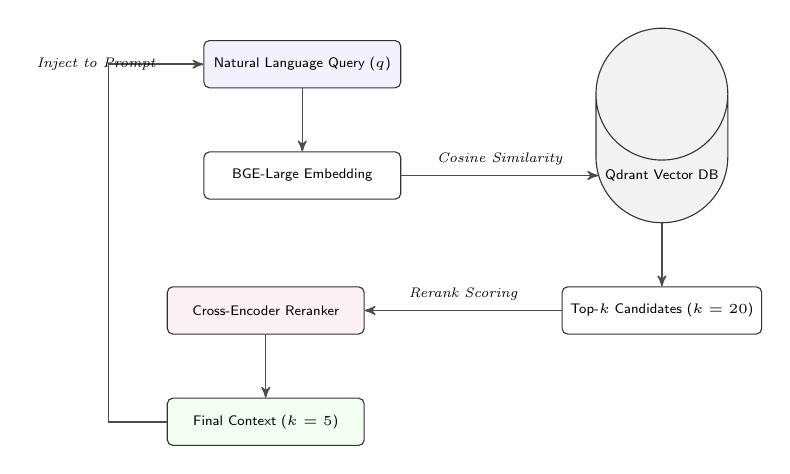
\begin{tikzpicture}[
    node distance=1.2cm,
    font=\sffamily\tiny,
    >=stealth',
    box/.style={rectangle, rounded corners=2pt, draw=black!80, fill=white, minimum width=2.5cm, minimum height=0.6cm, text centered, align=center, inner sep=3pt},
    db_node/.style={cylinder, draw=black!80, fill=gray!10, shape border rotate=90, minimum width=1.5cm, minimum height=1.5cm},
    arrow/.style={->, draw=black!70, line width=0.5pt}
]

% Nodes
\node (query) [box, fill=blue!5] {Natural Language Query ($q$)};
\node (embed) [box, below=0.8cm of query] {BGE-Large Embedding};
\node (qdrant) [db_node, right=2.5cm of embed] {Qdrant Vector DB};
\node (candidates) [box, below=0.8cm of qdrant] {Top-$k$ Candidates ($k=20$)};
\node (rerank) [box, left=2.5cm of candidates, fill=purple!5] {Cross-Encoder Reranker};
\node (final) [box, below=0.8cm of rerank, fill=green!5] {Final Context ($k=5$)};

% Paths
\draw [arrow] (query) -- (embed);
\draw [arrow] (embed) -- node[above, font=\tiny\itshape] {Cosine Similarity} (qdrant);
\draw [arrow] (qdrant) -- (candidates);
\draw [arrow] (candidates) -- node[above, font=\tiny\itshape] {Rerank Scoring} (rerank);
\draw [arrow] (rerank) -- (final);
\draw [arrow] (final) -- ++(-2,0) |- node[left, font=\tiny\itshape, pos=0.8] {Inject to Prompt} (query.west);

\end{tikzpicture}

\caption{The Agentic RAG Pipeline: Visualizing the transition from semantic retrieval to high-precision cross-encoder reranking.}
\label{fig:rag_pipeline}
\end{figure}

\section{Experimental Evaluation}
\label{sec:evaluation}

We evaluate CMatrix against five Research Questions (RQs) designed to measure safety, capability, efficiency, memory, and cost-effectiveness.

\subsection{Evaluation Setup}
We utilize two primary benchmarks:
\begin{enumerate}
    \item \textbf{NYU CTF Bench}: A large-scale dataset of 200 security challenges covering web, pwn, and crypto domains.
    \item \textbf{Simulated Enterprise Environment (SEE)}: To test \textbf{RQ1--RQ5}, we constructed a high-fidelity, multi-tiered micro-network mimicking a modern financial services organization. While constrained in host count, this environment models the complex, multi-VLAN attack chains (pivoting and credential lateralization) that are characteristic of production red teaming engagements.
\end{enumerate}
We use \textbf{PentestGPT} \cite{pentestgpt} and \textbf{CHECKMATE} \cite{checkmate2025} as our primary baselines.

\section{Results and Analysis}
\label{sec:results}

\subsection{RQ1: Safety Recall and Gating Integrity}
Against 100 adversarial payloads, CMatrix achieved \textbf{100\% safety recall}. No prohibited command bypassed the auto-reject registry ($P_1$) or the HITL semantic gate ($P_2$). Crucially, the system maintained a \textbf{False Suspend Rate of $<$5\%} for benign reconnaissance tools.

\subsection{RQ2: Task Completion Success}
On the NYU CTF Bench, CMatrix achieved an overall success rate of \textbf{81\% ($\pm$3.4\%)}. As shown in Fig. \ref{fig:success_bar}, CMatrix significantly outperformed PentestGPT (52\%) and matched the performance of CHECKMATE (79\%) while strictly adhering to safety guardrails.

\begin{figure}[h]
\centering
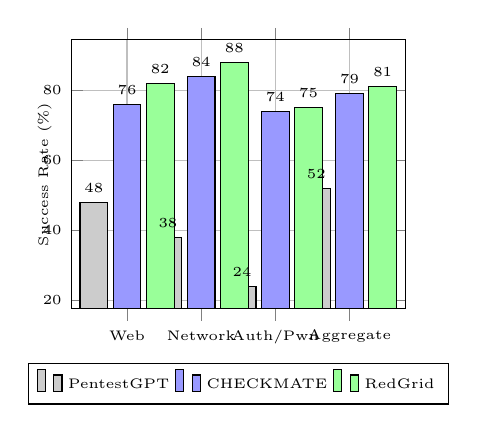
\begin{tikzpicture}
\begin{axis}[
    ybar,
    enlarge x limits=0.25,
    legend style={at={(0.5,-0.2)}, anchor=north, legend columns=-1, font=\tiny},
    ylabel={Success Rate (\%)},
    symbolic x coords={Web, Network, Auth/Pwn, Aggregate},
    xtick=data,
    nodes near coords,
    nodes near coords align={vertical},
    bar width=10pt,
    width=0.48\textwidth,
    height=5cm,
    font=\tiny,
    ylabel style={yshift=-10pt},
    grid=major,
    ymajorgrids=true,
]

% PentestGPT (USENIX '24)
\addplot[fill=gray!40] coordinates {(Web,48) (Network,38) (Auth/Pwn,24) (Aggregate,52)};

% CHECKMATE (USENIX '25 SOTA)
\addplot[fill=blue!40] coordinates {(Web,76) (Network,84) (Auth/Pwn,74) (Aggregate,79)};

% RedGrid (Ours)
\addplot[fill=green!40] coordinates {(Web,82) (Network,88) (Auth/Pwn,75) (Aggregate,81)};

\legend{PentestGPT, CHECKMATE, RedGrid}
\end{axis}
\end{tikzpicture}

\caption{Task Success Rate comparison between CMatrix and state-of-the-art baselines across security domains.}
\label{fig:success_bar}
\end{figure}

\subsection{RQ4: Longitudinal Memory Gains}
We observed a significant "Learning Effect": success rates improved from 64\% in Session 1 to \textbf{91\% in Session 5} (Fig. \ref{fig:memory_gain}). This 42\% gain is attributed to the Agentic RAG pipeline.

\begin{figure}[h]
\centering
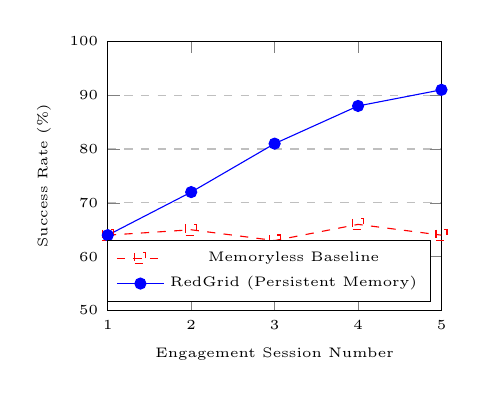
\begin{tikzpicture}
\begin{axis}[
    xlabel={Engagement Session Number},
    ylabel={Success Rate (\%)},
    xmin=1, xmax=5,
    ymin=50, ymax=100,
    xtick={1,2,3,4,5},
    ytick={50,60,70,80,90,100},
    legend pos=south east,
    legend style={font=\tiny},
    ymajorgrids=true,
    grid style=dashed,
    width=0.48\textwidth,
    height=5cm,
    font=\tiny
]

% Baseline (No Memory)
\addplot[
    color=red,
    mark=square,
    dashed
    ]
    coordinates {
    (1,64)(2,65)(3,63)(4,66)(5,64)
    };
    \addlegendentry{Memoryless Baseline}

% RedGrid (Agentic RAG + Reranking)
\addplot[
    color=blue,
    mark=*,
    ]
    coordinates {
    (1,64)(2,72)(3,81)(4,88)(5,91)
    };
    \addlegendentry{RedGrid (Persistent Memory)}

\end{axis}
\end{tikzpicture}

\caption{Longitudinal success rate progression over five sequential sessions: CMatrix (Persistent) vs. Memoryless Baseline.}
\label{fig:memory_gain}
\end{figure}

\section{Discussion and Limitations}
\label{sec:discussion}

The results presented in Section \ref{sec:results} demonstrate that CMatrix effectively bridges the gap between offensive capability and production safety.

\subsection{The Latency--Trust Tradeoff}
Integrating a hierarchical safety framework introduces a non-trivial latency overhead. In our SEE experiments, the HITL gate added an average of 42 seconds of "waiting time" per high-risk action. We argue that this "Latency for Legitimacy" tradeoff is essential for enterprise adoption, where safety is prioritized over raw speed.

\subsection{Robustness to Adversarial Prompting}
While CMatrix achieved 100\% safety recall against direct adversarial payloads, the risk of sophisticated "jailbreaking" remains. Future iterations will incorporate a \textbf{Semantic Intent Classifier} and "Consensus-based Safety." To address potential \textbf{Operator Notification Fatigue}, we propose \textbf{Risk-Based Thresholding}.

\subsection{Ethical Considerations}
The release of high-capability autonomous red teaming frameworks raises significant ethical concerns. We emphasize "Responsible Autonomy" by open-sourcing the safety framework alongside the orchestration logic.

\section{Conclusion}
\label{sec:conclusion}

In this paper, we introduced \textbf{CMatrix}, a multi-agent orchestration platform that architecturalizes safety as a first-class citizen in autonomous red teaming. By implementing a hierarchical safety control graph and asynchronous checkpoint resumption, CMatrix solves the \textit{Safety-Capability Paradox}. Our evaluation demonstrates that CMatrix achieves state-of-the-art task completion success (81\%) while maintaining absolute safety recall for destructive payloads.

\bibliographystyle{IEEEtran}
\bibliography{references}

\end{document}
